%Interpolation-Classes
%Interpolation
\rule{\textwidth}{0.4pt}
\class{Interpolation}
public abstract class Interpolation
\\\\
\begin{minipage}{0.5\textwidth}
    \begin{figure}[H]
        {\centering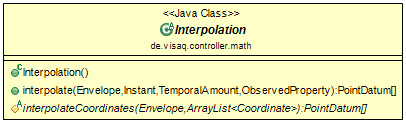
\includegraphics[width=0.95\textwidth]{media/backend/controller/classes/Interpolation.png}}
    \end{figure}
    \end{minipage} \hfill
\begin{minipage}{0.5\textwidth}
    Die abstrakte Klasse Interpolation stellt Interpolationsalgorithmen da, mit welchen die Sensordaten aus der Datenbank der \gls{SensorThings API} interpoliert werden können.
    Die Algorithmen interpolieren die Messpunkte nicht durchgehend sondern nur an gleichmäßig verteilten Punkten.
\end{minipage}

Methoden:
\begin{itemize}
    \item \emph{public Interpolation()}
    \constructorDescription{Interpolation}
    \item \emph{public PointDatum[] interpolate(Envelope envelope, Instant time, TemporalAmount range, ObservedProperty observedProperty)}
    Die Methode interpoliert alle Daten zu dem angegebene ObservedProperty, in einem beschränkten Bereich zu einem festem Zeitpunkt.
    Zur Angabe des Zeitpunktes findet als Instanz der Java-eigenen Klasse java.time.Instant statt.
    Für die Angabe der Region wird die Klasse org.locationtech.jts.geom.Envelope verwendet.
    Diese Klasse Envelope stellt einen rechteckigen Bereich da.
    Das Attribut range gibt an, aus welchem zeitlichen Bereich die für die Interpolation berücksichtigten Messwerte stammen.
    \item \emph{protected abstract PointDatum[] interpolateCoordinates(Envelope envelope, ArrayList<Coordinate> coordinates)}
    Die Methode interpoliert Daten die im Attribut coordinates gegben sind.
    Das Attribut coordinates besteht aus einer Liste von org.locationtech.jts.geom.Coordinate Instanzen.
    Eine Instanz besteht hierbei aus den beiden Geo-Koordinaten udn einem Messwert an der definierten Stelle.
    Zudem wird eine org.locationtech.jts.geom.Envelope Instanz übergeben, die den zu Interpolierenden Bereich angibt.
    Die Rückgabe besteht aus einem Array von PointDatum Instanzen, die die interpolierten Werte abbilden.
\end{itemize}

%DefaultInterpolation
\rule{\textwidth}{0.4pt}
\class{DefaultInterpolation}
public class DefaultInterpolation extends Interpolation
\\\\
%\begin{minipage}{0.5\textwidth}
    \begin{figure}[H]
        {\centering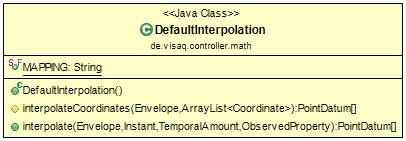
\includegraphics[width=0.7\textwidth]{media/backend/controller/classes/DefaultInterpolation.png}}
    \end{figure}
%\end{minipage} \hfill
%\begin{minipage}{0.5\textwidth}
    Die Klasse DefaultInterpolation implementiert den standart Interpolationsalgorithmus.
    Dieser Algorithmus verwendet hierfür Barnes Interpolation (siehe \url{https://en.wikipedia.org/wiki/Barnes_interpolation}).
    Diese Art der Interpolation kann besonders gut mit unregelmäßig verteilten Messpunkten umgehen.
    Barnes Interpolation wird speziell für die Interpolation von Wetterdaten verwendet, weswegen es für die hier interpolierten Werte sehr gut geignet ist.
    Für die Interpolation wird auf die Bibliothek org.geotools \url{https://geotools.org/} zurück gegriffen.
    Die Barnes Interpolation ist hier bereits als Klasse implementiert (\href{http://docs.geotools.org/latest/javadocs/org/geotools/process/vector/BarnesSurfaceInterpolator.html}{siehe}).
%\end{minipage}
\\
Attribute:
\begin{itemize}
    \item \emph{public static final String MAPPING} \mappingDescription
\end{itemize}
Methoden:
\begin{itemize}
    \item \emph{public DefaultInterpolation()}
    \constructorDescription{DefaultInterpolation}
    \item \emph{public PointDatum[] interpolate(Envelope envelope, Instant time, TemporalAmount range, ObservedProperty observedProperty)}
    Von der Klasse Interpolation geerbte Methode. Die methode wird hier um ein Mapping auf die Webschnittstelle der Spring-Applikation ergänzt.
   \item \emph{protected PointDatum[] interpolateCoordinates(Envelope envelope, ArrayList<Coordinate> coordinates)}
    Diese Methode wird von der Klasse Interpolation geerbt und hier mit der Barnes Interpolation implementiert.
\end{itemize}